\documentclass{article}
\usepackage[T1]{fontenc}
\usepackage{lmodern}
\usepackage{graphicx}
\usepackage{amsmath,amssymb}
\usepackage[a4paper,margin=2cm]{geometry}
\usepackage[absolute,overlay]{textpos}
\setlength{\TPHorizModule}{1mm}
\setlength{\TPVertModule}{1mm}
\usepackage[indonesian]{babel}
\usepackage{hyperref}
\setlength{\emergencystretch}{2em}
% unit: Halaman 33

\begin{document}

% === Halaman 33 (llm) ===

\vspace{70mm}

\begin{center}
{\Large S-box di dalam Rijndael}
\end{center}

% deskripsi: Tabel S-box yang digunakan dalam algoritma enkripsi Rijndael (AES), yang memetakan nilai input heksadesimal (baris dan kolom) ke nilai output heksadesimal.
% bbox normalisasi: [0.1300, 0.1100, 0.7600, 0.8300]
\begin{textblock*}{132.30mm}(27.30mm,32.67mm)
\noindent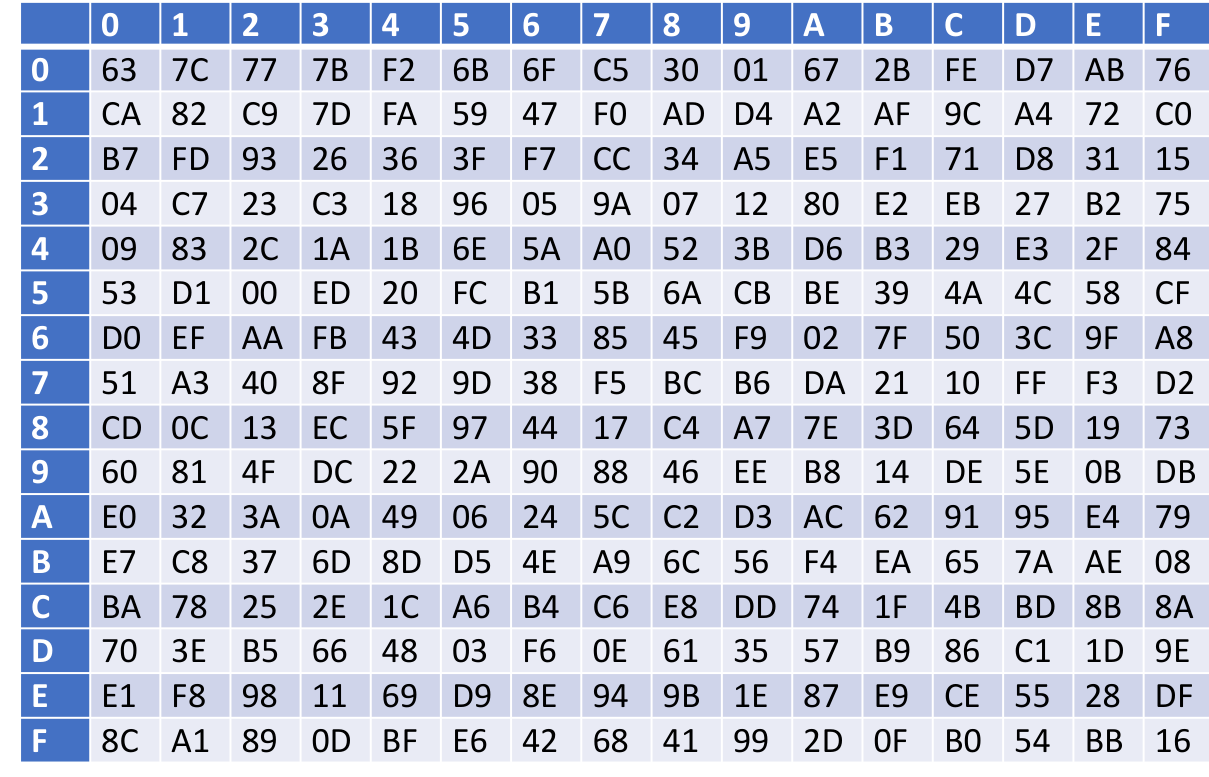
\includegraphics[width=132.30mm,height=213.84mm]{../../images/llm/page_033_img_01.png}%
\end{textblock*}

\end{document}
